%%
%% This is file `sample-acmlarge.tex',
%% generated with the docstrip utility.
%%
%% The original source files were:
%%
%% samples.dtx  (with options: `all,journal,bibtex,acmlarge')
%% 
%% IMPORTANT NOTICE:
%% 
%% For the copyright see the source file.
%% 
%% Any modified versions of this file must be renamed
%% with new filenames distinct from sample-acmlarge.tex.
%% 
%% For distribution of the original source see the terms
%% for copying and modification in the file samples.dtx.
%% 
%% This generated file may be distributed as long as the
%% original source files, as listed above, are part of the
%% same distribution. (The sources need not necessarily be
%% in the same archive or directory.)
%%
%%
%% Commands for TeXCount
%TC:macro \cite [option:text,text]
%TC:macro \citep [option:text,text]
%TC:macro \citet [option:text,text]
%TC:envir table 0 1
%TC:envir table* 0 1
%TC:envir tabular [ignore] word
%TC:envir displaymath 0 word
%TC:envir math 0 word
%TC:envir comment 0 0
%%
%% The first command in your LaTeX source must be the \documentclass
%% command.
%%
%% For submission and review of your manuscript please change the
%% command to \documentclass[manuscript, screen, review]{acmart}.
%%
%% When submitting camera ready or to TAPS, please change the command
%% to \documentclass[sigconf]{acmart} or whichever template is required
%% for your publication.
%%
%%
\documentclass[acmlarge]{acmart}
\usepackage{graphicx}
%%
%% \BibTeX command to typeset BibTeX logo in the docs
\AtBeginDocument{%
  \providecommand\BibTeX{{%
    Bib\TeX}}}

%% Rights management information.  This information is sent to you
%% when you complete the rights form.  These commands have SAMPLE
%% values in them; it is your responsibility as an author to replace
%% the commands and values with those provided to you when you
%% complete the rights form.
\setcopyright{acmlicensed}
\copyrightyear{2018}
\acmYear{2018}
\acmDOI{XXXXXXX.XXXXXXX}

%%
%% These commands are for a JOURNAL article.
\acmJournal{POMACS}
\acmVolume{37}
\acmNumber{4}
\acmArticle{111}
\acmMonth{8}

%%
%% Submission ID.
%% Use this when submitting an article to a sponsored event. You'll
%% receive a unique submission ID from the organizers
%% of the event, and this ID should be used as the parameter to this command.
%%\acmSubmissionID{123-A56-BU3}

%%
%% For managing citations, it is recommended to use bibliography
%% files in BibTeX format.
%%
%% You can then either use BibTeX with the ACM-Reference-Format style,
%% or BibLaTeX with the acmnumeric or acmauthoryear sytles, that include
%% support for advanced citation of software artefact from the
%% biblatex-software package, also separately available on CTAN.
%%
%% Look at the sample-*-biblatex.tex files for templates showcasing
%% the biblatex styles.
%%

%%
%% The majority of ACM publications use numbered citations and
%% references.  The command \citestyle{authoryear} switches to the
%% "author year" style.
%%
%% If you are preparing content for an event
%% sponsored by ACM SIGGRAPH, you must use the "author year" style of
%% citations and references.
%% Uncommenting
%% the next command will enable that style.
%%\citestyle{acmauthoryear}


%%
%% end of the preamble, start of the body of the document source.
\begin{document}

%%
%% The "title" command has an optional parameter,
%% allowing the author to define a "short title" to be used in page headers.
\title{Comparing Gaze and Controller Input for Task Management in Virtual Reality Environments}

%%
%% The "author" command and its associated commands are used to define
%% the authors and their affiliations.
%% Of note is the shared affiliation of the first two authors, and the
%% "authornote" and "authornotemark" commands
%% used to denote shared contribution to the research.
\author{Patrick McGuire}
\email{patrick.mcguire@colostate.edu}
\affiliation{%
  \institution{Colorado State University}
  \city{Fort Collins}
  \state{Colorado}
  \country{USA}
}

\author{Noah Larchick}
\email{nlarchic@colostate.edu}
\affiliation{%
  \institution{Colorado State University}
  \city{Fort Collins}
  \state{Colorado}
  \country{USA}
}

\author{Cole Nading}
\affiliation{%
 \institution{Colorado State University}
 \city{Fort Collins}
 \state{Colorado}
 \country{USA}}
\email{cole.nading@colostate.edu}

\author{Braden Stauffer}
\affiliation{%
 \institution{Colorado State University}
 \city{Fort Collins}
 \state{Colorado}
 \country{USA}}
\email{bstauff@colostate.edu}

%\author{Valerie B\'eranger}
%\affiliation{%
%  \institution{Inria Paris-Rocquencourt}
%  \city{Rocquencourt}
%  \country{France}
%}


%%
%% By default, the full list of authors will be used in the page
%% headers. Often, this list is too long, and will overlap
%% other information printed in the page headers. This command allows
%% the author to define a more concise list
%% of authors' names for this purpose.
\renewcommand{\shortauthors}{Trovato et al.}

%%
%% The abstract is a short summary of the work to be presented in the
%% article.
\begin{abstract}
As extended reality technologies become more prevalent in everyday life, understanding how users interact with task management systems in immersive environments is increasingly important. This study evaluates user interface design in virtual reality by comparing two interaction modalities—gaze-based and controller-based—in a VR task list application. A virtual grocery shopping task was developed in Unreal Engine 5 and tested using the Meta Quest 2 headset. Participants completed the same task using both input methods, allowing for direct performance comparison. Results indicate that controller-based interaction provided significantly faster and more accurate task completion, while gaze-based input offered a more intuitive and hands-free experience at the cost of precision. These findings highlight key trade-offs between efficiency and usability in immersive environments and contribute to ongoing research in extended reality by informing design decisions for future productivity-focused XR applications.
\end{abstract}


%%
%% The code below is generated by the tool at http://dl.acm.org/ccs.cfm.
%% Please copy and paste the code instead of the example below.
%%
%\begin{CCSXML}
%<ccs2012>
% <concept>
%  <concept_id>00000000.0000000.0000000</concept_id>
%  <concept_desc>Do Not Use This Code, Generate the Correct Terms for Your Paper</concept_desc>
%  <concept_significance>500</concept_significance>
% </concept>
% <concept>
%  <concept_id>00000000.00000000.00000000</concept_id>
%  <concept_desc>Do Not Use This Code, Generate the Correct Terms for Your Paper</concept_desc>
%  <concept_significance>300</concept_significance>
% </concept>
% <concept>
%  <concept_id>00000000.00000000.00000000</concept_id>
%  <concept_desc>Do Not Use This Code, Generate the Correct Terms for Your Paper</concept_desc>
%  <concept_significance>100</concept_significance>
% </concept>
% <concept>
%  <concept_id>00000000.00000000.00000000</concept_id>
%  <concept_desc>Do Not Use This Code, Generate the Correct Terms for Your Paper</concept_desc>
%  <concept_significance>100</concept_significance>
% </concept>
%</ccs2012>
%\end{CCSXML}

%\ccsdesc[500]{Do Not Use This Code~Generate the Correct Terms for Your Paper}
%\ccsdesc[300]{Do Not Use This Code~Generate the Correct Terms for Your Paper}
%\ccsdesc{Do Not Use This Code~Generate the Correct Terms for Your Paper}
%\ccsdesc[100]{Do Not Use This Code~Generate the Correct Terms for Your Paper}

%%
%% Keywords. The author(s) should pick words that accurately describe
%% the work being presented. Separate the keywords with commas.
%\keywords{Do, Not, Us, This, Code, Put, the, Correct, Terms, for,
%  Your, Paper}

\received{20 February 2007}
\received[revised]{12 March 2009}
\received[accepted]{5 June 2009}

%%
%% This command processes the author and affiliation and title
%% information and builds the first part of the formatted document.
\maketitle

\section{Introduction}
In an increasingly digital world, the integration of extended reality into our everyday lives is a promising avenue for promoting productivity and overall user experience. Our project aims to explore this potential by comparing the efficiency of both augmented reality and virtual reality interfaces with traditional smartphones list applications across realistic scenarios; potential scenarios ranging from grocery shopping to outdoor activities like fishing or skiing. We will use metrics such as error rate, task completion time, and user satisfaction discovered through user surveys, we aim to further our understanding of whether virtual and augmented reality can offer a more intuitive and enjoyable experience for managing routine activities.

This project thus lies within the area of user interface design, interaction, and experience within extended reality. Many user interface design considerations within a 2D environment are challenged when designing for a 3D interface such as virtual reality \cite{Xie_2023}. With that consideration and the large interest in virtual reality tools, there are many different avenues for designing such an interface within virtual reality. Our project seeks to incorporate and compare many of these for the purpose of improving user interactivity with our virtual reality task list implementation. Further, with virtual reality seeing large growth in use cases for different fields such as education \cite{Liu25112024}, a virtual reality task list could then see expansion into many different areas.

As day-to-day life becomes more and more reliant on digital technology, users increasingly rely on things such as task management to stay organized in both personal and professional settings. Traditional mobile apps offer a good solution with a structured way to manage tasks, but they often lack spatial context or hands-free interaction. By investigating whether AR interfaces can streamline task handling and improve engagement, our study contributes to a growing conversation around how emerging technologies can enhance cognitive workflows and simplify digital organization. 

\section{Previous Work}
Here we introduce previous findings on the success of task lists, virtual reality, and interaction techniques. We dive deeper into their interconnectedness and performance when used in tandem.

\subsection{Interaction techniques in VR}
In a 2024 study on effective task switching, a group of researchers looked at the concept of spatial gaze markers to assist users in augmented reality to better transition between tasks \cite{10.1145/3613904.3642811}. Although this study primarily looked at tasks as an action, this research can also be applied to the idea of a task list by using gaze markers when returning to a task description within a list. Another study performed in 2023 looked at how using AR devices to display a list can enhance a warehouse work task \cite{app132212222}. In the study they compared paper lists to augmented reality lists and how they can be best represented to enhance work performance. The analysis on user performance through having users complete a given task can help give insight as to how we may best test our project. A 2024 study compared some of the most popular interaction techniques when using head mounted displays such as for AR or VR \cite{10.1145/3698146} This research is primarily interesting as all of these interaction techniques can be applied to a task list. This helps our experiment as we don’t need to repeat the study by over-analyzing specific interaction techniques and instead apply the ones already studied.

Extending off the idea of the many different methods of input for a virtual reality user interface, the 2019 research study, "Comparison of Gaze Cursor Input Methods for Virtual Reality Devices", looks at one specific method in particular, gaze cursors. The article states that this gaze input method is used mainly as a replacement for a controller \cite{ctx39340979090003361}. This is of large interest to our research and prototype as a hands-free virtual reality task list may be preferred to a user who is actively performing a set of duties. They compared the gaze selection method with a manual selection method where the user pressed a separate button while the cursor was placed on the object \cite{ctx39340979090003361}. They thus found that the manual selection mode had a faster rate of task completion, but had a higher error rate than the gaze input method, with it being five times higher \cite{ctx39340979090003361}. Further, they chose to compare different timings for the gaze selection methods, to simplify this concept, these timings roughly controlled how long the users had to look at a button for it to be selected \cite{ctx39340979090003361}. The timings compared were measured in seconds being 1, 1.5, and 2. This is important to our project and prototype as they found 1 second gaze duration to perform better than the other options when the users did the given task \cite{ctx39340979090003361}. Within our prototype we will thus seek to use a similar duration, or lower as 1-s was the lowest time the study looked it, this indicates that even lower durations may provide better results. Finally, the study states that the findings may be of uses in tasks with a requirement of repeated selections, such as a keyboard \cite{ctx39340979090003361}. This may provide an option for the most optimal solution to creating tasks within virtual reality alongside being useful as a way to select tasks out of a list.

\subsection{Implications of Virtual Reality}
Recent work by Gronowski et al. (2024) compared user performance between AR and VR conditions in data visualization tasks and found that VR significantly outperformed AR in terms of task completion time, effectiveness, and satisfaction \cite{gronowski2024}. Participants also reported lower cognitive load in VR, suggesting that full immersion can benefit complex task handling—even at the expense of real-world context. This insight may indicate similar performance advantages in our own VR task list prototype. 

Meanwhile, Jacobsen et al. (2022) validated the realism of VR simulations by showing no significant difference in price recall between participants shopping in a physical grocery store and those in a VR replica \cite{jacobsen2022}. This affirms the ecological validity of using VR for everyday activities like shopping—relevant to our experiment where VR grocery tasks are used to measure interface performance.  

A 2021 research paper, "Information retrieval interfaces in virtual reality-A scoping review focused on current generation technology", compared information retrieval interfaces in virtual reality to more traditional methods, primarily looking at research papers on different virtual reality methods and how they can be applied to this kind of system. Citing that the experience has been mostly the same since their creation, with search interfaces, speech recognition, etc \cite{10.1371/journal.pone.0246398}. Although this study looked at interfaces for storing and retrieving data from digital databases, many of these same concepts can be applied to a virtual reality task list. This is due to many of the user-interface concepts being easy to apply from the usability of a information retrieval system to a system for storing and retrieving tasks. Although the study looked at many different processes and theories for performing these tasks in virtual reality, they found that most of them proved to have significantly higher user performance in both speed and quality \cite{10.1145/3698146}. This may give an indication of results we might see within our own study when comparing traditional task lists to those represented within a virtual reality system. Further, the study cites that due to the wide range of sources for these systems built in virtual reality, it would be best to design a working prototype. Citing that a thorough and open-minded study with a proper baseline would be important \cite{10.1371/journal.pone.0246398}. Although this study looked at a different topic of virtual reality user interfaces, this is adjacent to our prospective area and we will perform these requirements on our prototype.

Pini et al. (2023) demonstrated AR’s potential in improving grocery decision-making by showing that real-time nutrition overlays influenced participants to choose healthier options \cite{pini2023}. This supports our design decision to use AR visual cues in a shopping context and highlights the interface’s role in enhancing awareness and decision quality.

\subsection{Task List Effectiveness}
While our project focuses primarily on virtual reality and its implications for task management, a critical aspect of the research lies in understanding real-world task list design. A 2004 study on task management and task list design revealed interesting results on optimal task list design choices and their corresponding completion rate values \cite{bellotti2004studies}. The study found that most people are quite effective at creating proper prioritization on their task lists but fail to apply the proper effort to complete them when the time comes \cite{bellotti2004studies}. The study additionally found that task lists via email, paper print-out, and index-card had a lower complete-rate within a week. Contrasting this, notes in a notebook, vertical folders, and an open PC tab were the most effective. This component of the study specifically aligns with our project, in that our task list will most likely be formatted in the open PC tab format. Conclusive evidence from this study will likely be beneficial for the creation of our prototypes and the development of successful task lists in Virtual Reality. A 2005 study on human-robot interaction similarly found results around the use of a task-list in improving human management efficiency \cite{envarli2005task}. Mirroring earlier findings, the study demonstrated that a structured task-list significantly improved performance, particularly for users unfamiliar with the system: “[t]he results have shown that the task list produced improved performance when the users had little familiarity with the system” \cite{envarli2005task}. The participants valued the organization and prioritization provided by the task-list interface which was crucial to task completion. Compared to index cards the task list shown a 1+ minute time improvement to completion times during their study. Notably, in both studies the PC-tab format task-list, proved to be an effective organization solution for many test scenarios. Given these results, a VR-based task-list could similarly improve performance in digital simulations by providing clear task structure and guidance.

Task lists have been shown to improve completion efficiency for various tasks, though many studies define shortcomings of the task list in their individual study environments. For instance, a 2015 study on mobile collaborative task lists found efficiency improvements, yet adoption rates remained low due to key limitations \cite{michelson2015mobile}. While the task list proved easy to use and was helpful in the completion of 89\% of tasks, the need for additional login steps and physical proximity between users reduced its effectiveness and practicality. The users deemed physical sticky-notes to be a better solution to the issue. Two main shortcomings were identified in the study: (1) lack of integration with the existing software, and (2) redundant communication provided the users’ close physical proximity \cite{roemer2005redundancy}. In contrast, our study and integration of a task list, the virtual environment does not have additional software dependencies, nor does it involve unnecessary collaboration. By addressing these limitations, our study approach may lead to greater efficiency gains in task completion specifically in a virtual environment.

\subsection{Personal Productivity in AR/VR} While academic research has laid the groundwork for understanding interaction techniques in extended reality, most commercial efforts in AR and VR have focused on large-scale, enterprise, or entertainment applications. For example, Microsoft’s HoloLens 2 is widely used in industrial training, remote assistance, and medical visualization, emphasizing team-based collaboration and enterprise workflows rather than personal organization or task management \cite{microsoft_hololens_2023}. Meta’s Horizon Workrooms and Quest platforms are largely designed for immersive social interaction, gaming, and virtual collaboration, rather than structured, solo task execution \cite{meta_horizon_workrooms_2021}. These platforms showcase the broad potential of XR, but they often overlook the needs of individual users seeking to manage their everyday responsibilities—such as grocery shopping, packing, or tracking to-dos—within immersive environments. Additionally, prior studies tend to focus more on individual input techniques- such as gaze, gesture, or controller-based interactions- in isolation rather than comparing them in one single interface. Our project addresses this gap by developing a VR task list prototype that integrates multiple input modalities and supports common productivity actions, such as creating, selecting, and reordering tasks. By evaluating performance and user preference in realistic scenarios, we aim to explore how extended reality can enhance personal productivity through intuitive and immersive design. 

\section{Methodology}
This study seeks to analyze different extended reality approaches to user interface design when applied to creating a task list. Due to the broad area of this topic and the multiple applicable approaches, we created a prototype that integrates three interaction modalities- controller-based, gaze-based, and gesture- based – to compare their effectiveness. This enables us to then compare the methods against one another in an environment where the user has the power to use whatever method feels most appropriate, simulating real-world flexibility and personalization.  

We chose to develop our prototype in virtual reality to streamline testing and maintain ecological validity. By virtualizing the different real world tasks we asked our participants to perform, we avoid complications and large time requirements that would arise in a purely augmented reality approach. Furthermore, by replicating the real tasks in virtual reality, we believe these results are still useful to an augmented reality design space. 

\subsection{Participants} 
We recruited 8 participants (7 male, 1 female) between the ages of 21-24 from the university community. All participants volunteered and provided informed consent before beginning the study. To account for possible familiarity bias, all participants selected had a similar level of experience with virtual reality systems and smartphone- based task lists. This demographic information helps ensure the results reflect typical behavior under realistic conditions

\subsection{Prototype Development} 

We created our task-list prototype using Unreal engine and performed testing with the Meta Quest 2 headset. Virtual reality was chosen as the extended reality format used for testing due to allowing us to create and simulate different physical environments for performing tasks such as a grocery store. Virtual reality allows us to implement these real-world situations more easily in an isolated environment which provided a better context for testing user interaction especially when contrasted with the increased complexity of using augmented reality. 

The input modalities we selected to use were not only because of their relevance in prior research, but also for their practical implementation with the Meta Quest 2. VR development using the Unreal Engine blueprint system allows us to rapidly create prototypes for gaze, gesture, and controller-based interactions without requiring much low-level programming. The prototype integrates Meta’s XR Interaction SDK, which provides built in support for hand tracking and gesture recognition. Additionally, with the simplicity of the virtual environments in Unreal Engine, we were able to create a mock grocery store to simulate the natural task execution. This allows us to get an accurate evaluation of interaction performance under conditions that mimic real-world scenarios. 

The prototype incorporates three primary input methods which are based on the previous research: 

\subsubsection {Controller-Based Selection/Interaction:} 

With this method, users are able to interact with the task list, specifically items in the task list, using handheld virtual reality controllers. We chose to use the Quest Touch controllers as these came with the Quest 2 headset and were readily available. This interaction method replicates pointer-based interaction techniques, which gave us a baseline from previous work of which to go off \cite{10.1117/12.497665}. 

\subsubsection{Gaze-Based Selection/Interaction:} This method enables users to be able to interact with items in the task listen through a gaze-based cursor. Based on previous research and work, selecting items is accomplished by looking at them for a fixed gaze duration \cite{ctx39340979090003361}. Also, accordingly with the previous research’s findings, we set to gaze duration to highlight with gaze and select with trigger \cite{ctx39340979090003361}. 

\subsection{Procedure}

To evaluate the prototype, we conducted a user study where participants performed a simulated grocery shopping task within a virtual reality environment as seen in figure \ref{fig:store}. Each participant completed the same task twice under different input conditions: once using gaze-based interaction exclusively and once using controller-based interaction exclusively. The controller input utilized a beam-style pointing method via Meta Quest 2’s handheld controllers. This structure allowed for a controlled comparison between the two input modalities.

\begin{figure}
    \centering
    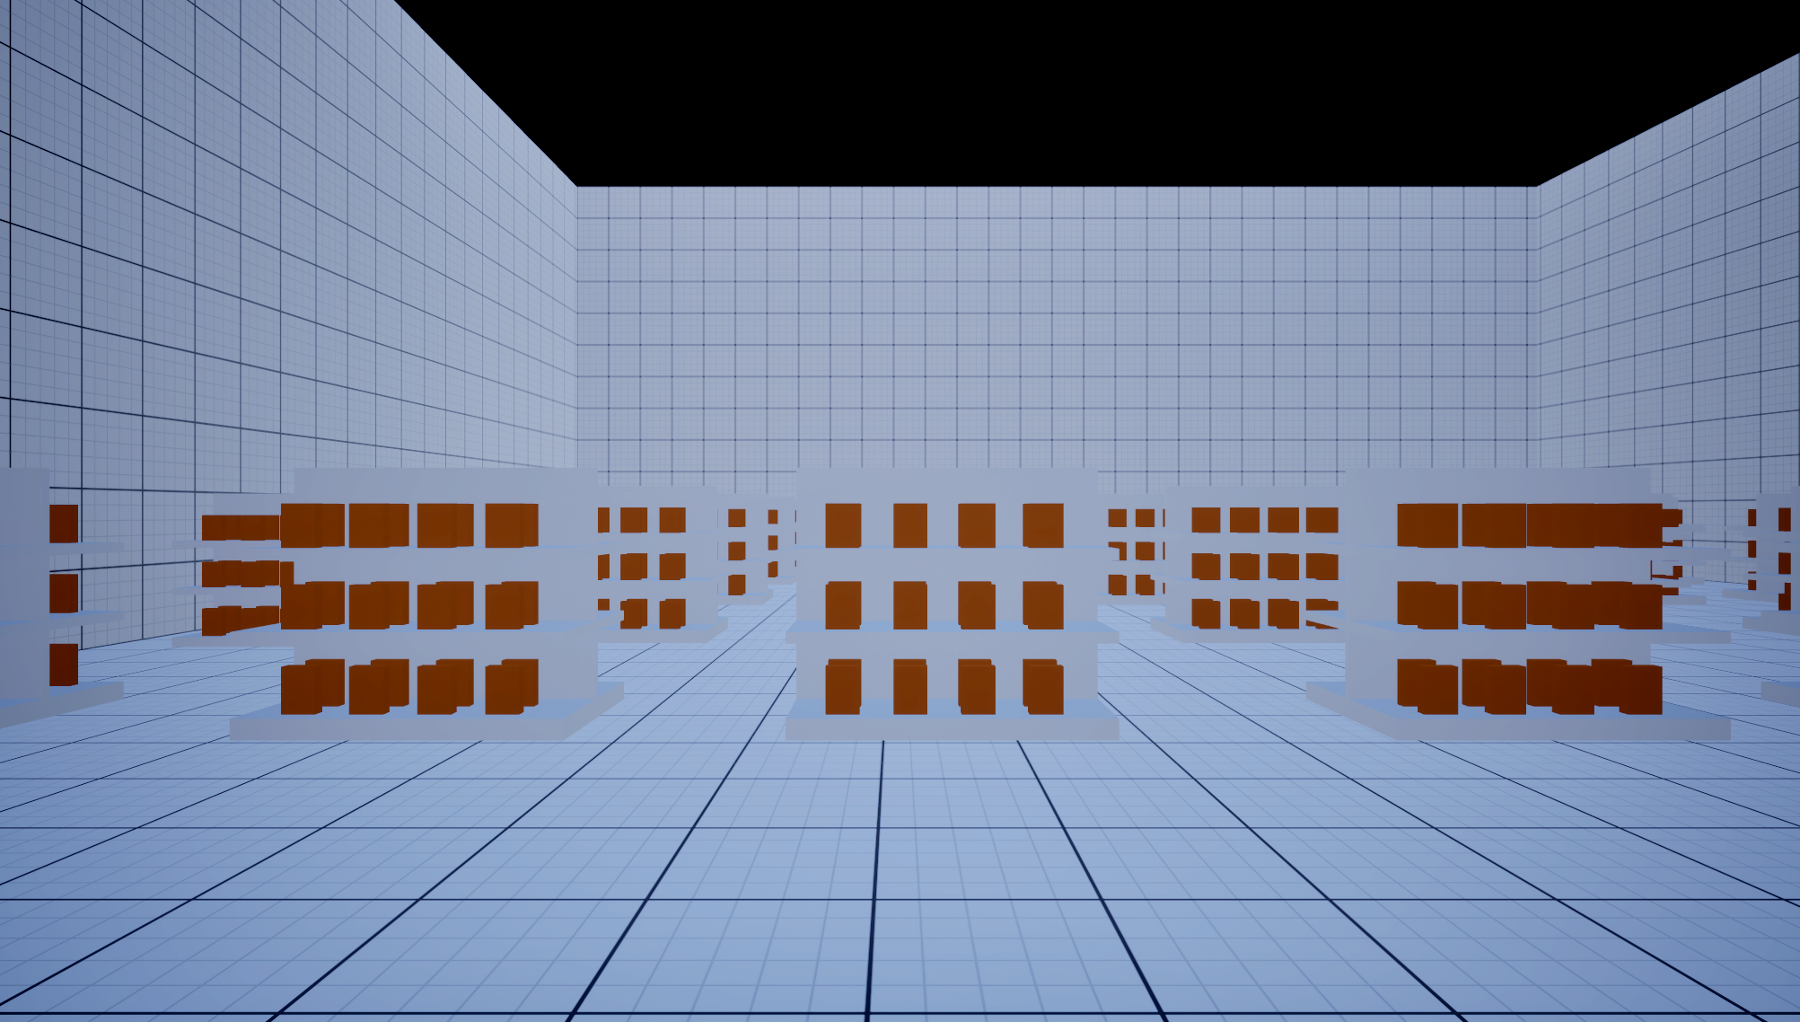
\includegraphics[width=1\linewidth]{VRStorePreview.png}
    \caption{Preview of VR store}
    \label{fig:store}
\end{figure}

Before beginning the tasks, each participant received a brief tutorial on the VR environment and both interaction methods to minimize bias caused by varying levels of VR experience. The task involved navigating a virtual grocery store, locating five distinct grocery items (differentiated by color and shape), and checking them off a virtual task list. The list interface could be accessed via the participant's wrist using controller input.

In the gaze-only trial, participants used a fixed-duration gaze cursor (highlighting a selection with gaze and trigger with a controller) to make selections and check off items. In the controller-only trial, participants used a laser pointer-style beam emitted from the controller to select and interact with list items. Input modality switching was disabled during each trial to preserve experimental control.

System logs recorded all user interactions, including task completion time, selection events, and any errors such as incorrect or accidental selections. After completing both trials, participants filled out a post-task survey comparing the two input methods. The survey included Likert-scale questions assessing ease of use, physical and cognitive effort, confidence in selections, and overall enjoyment, along with open-ended prompts for qualitative feedback.

Each session lasted approximately 20 minutes, including the tutorial, both input trials, and the follow-up survey.

\subsection{Measurements and Evaluation}

During and after the participant tests of our prototype, we collected both quantitative and qualitative data to evaluate user interaction. Quantitative metrics included task completion time and error rate, while qualitative feedback was gathered through Likert-scale questions assessing ease of use, physical and cognitive effort, confidence in selections, and overall enjoyment. Open-ended prompts further encouraged participants to describe any confusion, interaction preferences, and how they might use such a system in their daily lives.

\subsubsection{Task completion time:} How long a user takes to complete a specific task on the list as well as the overall completion time of all items on the task-list. 

\subsubsection{Error Rate:} The number of times where a user selects the wrong task item such as accidental selections or deletions. 

\subsubsection{User Preference:} After the initial test, we asked each user to rate the interaction techniques as well as any open-ended feedback they would provide. Further, we asked the user if they have utilized task-lists on their smartphone before, and if-so, how their experience compares to using the prototype.

\subsection{The Data}
Data collected from each scenario will be statistically analyzed to determine whether the AR task list provides a significant advantage—or disadvantage—compared to traditional list interfaces. This approach enables us to assess AR's viability as a practical organizational tool and provide recommendations for future HCI designs.\\

The independent variable is the display modality (AR vs. smartphone), while the dependent variables include task completion time, error rate (missed or incorrect tasks), and user satisfaction (measured via post-task surveys). The AR prototype will incorporate interaction techniques and visual cues from prior research—such as spatial gaze markers for reorienting attention—along with new techniques we develop during the project. The study emphasizes hands-free or minimal interaction methods to maintain immersion in physical tasks.\\

Quantitative data that is collected during the study will be analyzed using paired sample t-tests to assess if there are any significant differences between the AR task list and the traditional smartphone-based task list. Since each participant completes a task using both systems, this allows us to control individual differences and just focus on the impact of the interface itself. Data will be recorded for each participant across both conditions and structured to enable direct comparisons of task performance. These tests will be performed using a specific Python script that allows us to compute t-statistics and p-values. A p–value less than 0.05 will indicate a significant difference between the two conditions, helping us evaluate whether AR interfaces provide measurable performance benefits over conventional mobile-based task lists. \\

In addition to performance data, qualitative feedback will be collected through the post-task surveys. Participants will respond to Likert-scaled questions addressing usability, comfort, and effectiveness, as well as open-ended questions about their overall experience with each system. These qualitative responses will be grouped into themes to provide more insight into user satisfaction, cognitive load, and overall preferences. By integrating statistical findings with qualitative insights, our evaluation provides a comprehensive assessment of the practicality and effectiveness of AR-based task list interfaces in everyday scenarios. 

\section{Results}

We evaluated the performance of two interaction modalities—gaze-based and controller-based input—during a virtual grocery shopping task in a VR environment. Each of the 8 participants completed the same task twice: once using gaze-based selection exclusively, and once using controller-based (beam pointer) interaction exclusively. Quantitative data was collected on task completion time and error rates, while qualitative data was gathered through post-task surveys.

\subsection{Task Completion Time}

Controller-based input yielded the fastest average task completion time across participants. The mean completion time for controller input was {69.1 seconds (SD = 7.4)}, compared to {85.6 seconds (SD = 10.2)} for gaze-based input. A paired samples t-test showed a statistically significant difference in completion time between the two conditions ({p} < 0.01), indicating that controller input enabled faster task execution.

\subsection{Error Rates}

Error rate was defined as the number of incorrect selections or missed items per session. Controller input again performed better, with an average error rate of {0.75 errors per session}, compared to {2.1 errors} for gaze-based interaction. Several participants noted that unintentional selections occasionally occurred while using gaze, especially when scanning the interface or shifting attention rapidly between items.

\subsection{User Preference and Feedback}

Survey results showed a clear participant preference for controller-based interaction. Seven out of eight users ranked the controller modality as both the most efficient and the easiest to use. Gaze-based interaction was generally described as intuitive and physically less demanding, but less precise and more prone to errors. Participants appreciated the hands-free nature of gaze interaction but emphasized that improved dwell-time calibration or confirmation feedback would enhance its usability.

\subsection{Summary}

Our results suggest that while gaze-based interaction offers a viable and intuitive hands-free option, controller-based input currently provides superior performance in terms of both speed and accuracy for VR-based task list interactions. These findings highlight the continued reliability of traditional controller interfaces while also pointing to the potential of gaze as a complementary or alternative method for specific use cases. 

\section{Implications and Future Work}

The findings from this study offer important implications for the design of task management systems in virtual reality environments. Our results suggest that while controller-based interaction continues to be the most efficient and precise method, gaze-based input holds promise for hands-free interaction in contexts where physical movement may be constrained or convenience is prioritized. Designers of XR productivity tools should consider incorporating both modalities, offering users the flexibility to choose their preferred interaction method depending on context and task complexity.

Additionally, this research reinforces the value of immersive, spatial user interfaces for list-based task management, which has traditionally been confined to 2D screens. The ability to integrate task lists directly into spatial environments opens new possibilities for workflows that blend the digital and physical worlds.

Future work should expand the participant pool to include a broader demographic range and varying levels of XR experience to enhance the generalizability of the results. Moreover, exploring hybrid interfaces that combine gaze with subtle controller or voice input may yield improved performance without sacrificing hands-free usability. Longitudinal studies evaluating user adaptation over time would also help uncover whether gaze-based systems become more efficient with practice. Finally, comparing interaction methods across more complex or collaborative tasks could provide further insight into how immersive UIs can scale to meet the needs of professional and high-stakes environments.

\section{Conclusion}
This study investigated the performance and usability of two interaction modalities, gaze-based and controller-based, for managing task lists in a virtual reality environment. By simulating a grocery shopping task in VR and evaluating user performance across both input methods, we found controller-based interaction significantly outperformed gaze-based interaction in both speed and accuracy. Participants completed tasks faster and with fewer errors when using the handheld controllers.

While gaze-based input was praised for its hands-free design and intuitiveness, it introduced selection delays and precision challenges that hindered task efficiency. These results emphasize the practicality and reliability of traditional controller input in productivity-focused VR applications, while also highlighting the potential of gaze interaction as a complementary method under specific conditions.

Our findings contribute to ongoing XR research by offering actionable insight into input modality design for task management systems. As VR continues to evolve, future work should explore adaptive gaze calibration, multimodal input switching, and longer-term use cases to determine how hands-free interaction can be optimized for broader adoption in everyday XR workflows.

\begin{acks}
Thanks for a great Semester!
\end{acks}

%%
%% The next two lines define the bibliography style to be used, and
%% the bibliography file.
\bibliographystyle{ACM-Reference-Format}
\bibliography{bib.bib}


%%
%% If your work has an appendix, this is the place to put it.
\appendix
\end{document}
\endinput
%%
%% End of file `sample-acmlarge.tex'.
